%  template.tex for Biometrics papers
%
%  This file provides a template for Biometrics authors.  Use this
%  template as the starting point for creating your manuscript document.
%  See the file biomsample.tex for an example of a full-blown manuscript.

%  ALWAYS USE THE referee OPTION WITH PAPERS SUBMITTED TO BIOMETRICS!!!
%  You can see what your paper would look like typeset by removing
%  the referee option.  Because the typeset version will be in two
%  columns, however, some of your equations may be too long. DO NOT
%  use the \longequation option discussed in the user guide!!!  This option
%  is reserved ONLY for equations that are impossible to split across 
%  multiple lines; e.g., a very wide matrix.  Instead, type your equations 
%  so that they stay in one column and are split across several lines, 
%  as are almost all equations in the journal.  Use a recent version of the
%  journal as a guide. 
%  
\documentclass[useAMS,usenatbib, referee]{biom_supp}
%
%  If your system does not have the AMS fonts version 2.0 installed, then
%  remove the useAMS option.
%
%  useAMS allows you to obtain upright Greek characters.
%  e.g. \umu, \upi etc.  See the section on "Upright Greek characters" in
%  this guide for further information.
%
%  If you are using AMS 2.0 fonts, bold math letters/symbols are available
%  at a larger range of sizes for NFSS release 1 and 2 (using \boldmath or
%  preferably \bmath).
% 
%  Other options are described in the user guide. Here are a few:
% 
%  -  If you use Patrick Daly's natbib  to cross-reference your 
%     bibliography entries, use the usenatbib option
%
%  -  If you use \includegraphics (graphicx package) for importing graphics
%     into your figures, use the usegraphicx option
% 
%  If you wish to typeset the paper in Times font (if you do not have the
%  PostScript Type 1 Computer Modern fonts you will need to do this to get
%  smoother fonts in a PDF file) then uncomment the next line
%  \usepackage{Times}
\usepackage{amsmath}

%Following 3 lines for Tikz
\usepackage{xr}
\usepackage{tikz}
\usepackage{tikzscale}
\usepackage{graphicx}
\usepackage{url}
\usetikzlibrary{shapes.geometric, arrows, positioning}
%%%%% PLACE YOUR OWN MACROS HERE %%%%%

\externaldocument{pers_schedules}

\def\bSig\mathbf{\Sigma}
\newcommand{\VS}{V\&S}
\newcommand{\tr}{\mbox{tr}}
%\renewcommand{\figurename}{Web Figure}
%\renewcommand{\tablename}{Web Table}

\renewcommand\thesection{Web Appendix \Alph{section}}

\makeatletter
\renewcommand{\fnum@figure}{Web Figure \thefigure}
\makeatother

%Single spacing for tables
\makeatletter
\AtBeginEnvironment{tabular}{%
  \def\baselinestretch{1}\@currsize}%
\makeatother

%\renewcommand{\thetable}{Web \arabic{table}}

\DeclareMathOperator{\argmax}{arg\,max}


\tikzstyle{startstop} = [rectangle, rounded corners, minimum width=3cm, minimum height=1cm,text centered, draw=black,text width = 5cm, fill=red!30]
\tikzstyle{io} = [trapezium, trapezium left angle=70, trapezium right angle=110, minimum width=2cm, minimum height=1cm, text centered, draw=black, fill=blue!30]
\tikzstyle{process} = [rectangle, minimum width=3cm, minimum height=1cm, text centered, text width = 3cm, draw=black, fill=orange!30]
\tikzstyle{process_wide_3pt5cm} = [rectangle, minimum width=3cm, minimum height=1cm, text centered, text width = 3.5cm, draw=black, fill=orange!30]
\tikzstyle{process_wide_5cm} = [rectangle, minimum width=3cm, minimum height=1cm, text centered, text width = 5cm, draw=black, fill=orange!30]
\tikzstyle{decision} = [diamond, minimum width=1cm, minimum height=1cm,text centered,text width = 2.25cm, draw=black, fill=green!30]
\tikzstyle{arrow} = [thick,->,>=stealth]


%  The rotating package allows you to have tables displayed in landscape
%  mode.  The rotating package is NOT included in this distribution, but
%  can be obtained from the CTAN archive.  USE OF LANDSCAPE TABLES IS
%  STRONGLY DISCOURAGED -- create landscape tables only as a last resort if
%  you see no other way to display the information.  If you do do this,
%  then you need the following command.

%\usepackage[figuresright]{rotating}

%%%%%%%%%%%%%%%%%%%%%%%%%%%%%%%%%%%%%%%%%%%%%%%%%%%%%%%%%%%%%%%%%%%%%

%  Here, place your title and author information.  Note that in 
%  use of the \author command, you create your own footnotes.  Follow
%  the examples below in creating your author and affiliation information.
%  Also consult a recent issue of the journal for examples of formatting.

\title[Web-based Supplementary Materials  for ``Personalized schedules'']
{Web-based Supplementary Materials for ``Personalized Schedules for Prostate Cancer Biopsies''}

%  Here are examples of different configurations of author/affiliation
%  displays.  According to the Biometrics style, in some instances,
%  the convention is to have superscript *, **, etc footnotes to indicate 
%  which of multiple email addresses belong to which author.  In this case,
%  use the \email{ } command to produce the emails in the display.

%  In other cases, such as a single author or two authors from 
%  different institutions, there should be no footnoting.  Here, use
%  the \emailx{ } command instead. 

%  The examples below corrspond to almost every possible configuration
%  of authors and may be used as a guide.  For other configurations, consult
%  a recent issue of the the journal.

%  Single author -- USE \emailx{ } here so that no asterisk footnoting
%  for the email address will be produced.

%\author{John Author\emailx{email@address.edu} \\
%Department of Statistics, University of Warwick, Coventry CV4 7AL, U.K.}

%  Two authors from the same institution, with both emails -- use
%  \email{ } here to produce the asterisk footnoting for each email address

%\author{John Author$^{*}$\email{author@address.edu} and
%Kathy Authoress$^{**}$\email{email2@address.edu} \\
%Department of Statistics, University of Warwick, Coventry CV4 7AL, U.K.}

%  Exactly two authors from different institutions, with both emails  
%  USE \emailx{ } here so that no asterisk footnoting for the email address
%  is produced.

%\author
%{John Author\emailx{author@address.edu} \\
%Department of Statistics, University of Warwick, Coventry CV4 7AL, U.K. 
%\and
%Kathy Author\emailx{anotherauthor@address.edu} \\
%Department of Biostatistics, University of North Carolina at Chapel Hill, 
%Chapel Hill, North Carolina, U.S.A.}

%  Three or more authors from same institution with all emails displayed
%  and footnoted using asterisks -- use \email{ } 

%\author{John Author$^*$\email{author@address.edu}, 
%Jane Author$^{**}$\email{jane@address.edu}, and 
%Dick Author$^{***}$\email{dick@address.edu} \\
%Department of Statistics, University of Warwick, Coventry CV4 7AL, U.K}

%  Three or more authors from same institution with one corresponding email
%  displayed

\author{Anirudh Tomer$^{1,*}$\email{atomer@erasmusmc.nl}, 
Daan Nieboer$^{2}$, 
Monique J. Roobol$^3$, \\
\textbf{Ewout W. Steyerberg}$^{\bmath{2}}$, 
\textbf{and Dimitris Rizopoulos}$^{\bmath{1}}$ \\ \\
$^{1}$Department of Biostatistics, Erasmus University Medical Center, the Netherlands \\
$^{2}$Department of Public Health, Erasmus University Medical Center, the Netherlands \\
$^{3}$Department of Urology, Erasmus University Medical Center, the Netherlands}


%  Three or more authors, with at least two different institutions,
%  more than one email displayed 

%\author{John Author$^{1,*}$\email{author@address.edu}, 
%Kathy Author$^{2,**}$\email{anotherauthor@address.edu}, and 
%Wilma Flinstone$^{3,***}$\email{wilma@bedrock.edu} \\
%$^{1}$Department of Statistics, University of Warwick, Coventry CV4 7AL, U.K \\
%$^{2}$Department of Biostatistics, University of North Carolina at 
%Chapel Hill, Chapel Hill, North Carolina, U.S.A. \\
%$^{3}$Department of Geology, University of Bedrock, Bedrock, Kansas, U.S.A.}

%  Three or more authors with at least two different institutions and only
%  one email displayed

%\author{John Author$^{1,*}$\email{author@address.edu}, 
%Wilma Flinstone$^{2}$, and Barney Rubble$^{2}$ \\
%$^{1}$Department of Statistics, University of Warwick, Coventry CV4 7AL, U.K \\
%$^{2}$Department of Geology, University of Bedrock, Bedrock, Kansas, U.S.A.}


\begin{document}

%  This will produce the submission and review information that appears
%  right after the reference section.  Of course, it will be unknown when
%  you submit your paper, so you can either leave this out or put in 
%  sample dates (these will have no effect on the fate of your paper in the
%  review process!)

\date{{\it Received October} 0000. {\it Revised February} 0000.  {\it
Accepted March} 0000.}

%  These options will count the number of pages and provide volume
%  and date information in the upper left hand corner of the top of the 
%  first page as in published papers.  The \pagerange command will only
%  work if you place the command \label{firstpage} near the beginning
%  of the document and \label{lastpage} at the end of the document, as we
%  have done in this template.

%  Again, putting a volume number and date is for your own amusement and
%  has no bearing on what actually happens to your paper!  

\pagerange{\pageref{firstpage}--\pageref{lastpage}} 
\volume{00}
\pubyear{0000}
\artmonth{December}

%  The \doi command is where the DOI for your paper would be placed should it
%  be published.  Again, if you make one up and stick it here, it means 
%  nothing!

\doi{10.1111/j.1541-0420.2005.00454.x}

%  This label and the label ``lastpage'' are used by the \pagerange
%  command above to give the page range for the article.  You may have 
%  to process the document twice to get this to match up with what you 
%  expect.  When using the referee option, this will not count the pages
%  with tables and figures.  

%  As usual, the \maketitle command creates the title and author/affiliations
%  display 

\maketitle

\label{firstpage}
%  If you are using the referee option, a new page, numbered page 1, will
%  start after the summary and keywords.  The page numbers thus count the
%  number of pages of your manuscript in the preferred submission style.
%  Remember, ``Normally, regular papers exceeding 25 pages and Reader Reaction 
%  papers exceeding 12 pages in (the preferred style) will be returned to 
%  the authors without review. The page limit includes acknowledgements, 
%  references, and appendices, but not tables and figures. The page count does 
%  not include the title page and abstract. A maximum of six (6) tables or 
%  figures combined is often required.''

%  You may now place the substance of your manuscript here.  Please use
%  the \section, \subsection, etc commands as described in the user guide.
%  Please use \label and \ref commands to cross-reference sections, equations,
%  tables, figures, etc.
%
%  Please DO NOT attempt to reformat the style of equation numbering!
%  For that matter, please do not attempt to redefine anything!

% !TEX root =  ../supplementary.tex

\section{Joint Model for Time to Event and Longitudinal Outcomes}
\label{web_sec : jm_framework}
We start with the definition of the joint modeling framework that will be used to fit a model to the available dataset, and then to plan biopsies for future patients. Let $T_i^*$ denote the true Gleason reclassification (referred to as GR hereafter) time for the $i$-th patient enrolled in an AS program. Let $S$ be the schedule of biopsies prescribed to this patient. The corresponding vector of time of biopsies is denoted by $T_i^S = \{T^S_{i0}, T^S_{i1}, \ldots, T^S_{i{N_i^S}}; T^S_{ij} < T^S_{ik}, \forall j<k\}$, where $N_i^S$ are the total number of biopsies conducted. Because of the periodical nature of biopsy schedules, $T_i^*$ cannot be observed directly and it is only known to fall in an interval $(l_i, r_i]$, where $l_i = T^S_{i{N_i^S - 1}}, r_i = T^S_{i{N_i^S}}$ if GR is observed, and $l_i = T^S_{i{N_i^S}}, r_i=\infty$ if GR is not observed yet. Further let $\bmath{y}_i$ denote the $n_i \times 1$  vector of PSA levels for the $i$-th patient. For a sample of $n$ patients the observed data is denoted by $\mathcal{D}_n = \{l_i, r_i, \bmath{y}_i; i = 1, \ldots, n\}$.

The longitudinal outcome of interest, namely PSA level, is continuous in nature and thus to model it the joint model utilizes a linear mixed effects model (LMM) of the form:
\begin{equation*}
\begin{split}
y_i(t) &= m_i(t) + \varepsilon_i(t)\\
&=\bmath{x}_i^T(t) \bmath{\beta} + \bmath{z}_i^T(t) \bmath{b}_i + \varepsilon_i(t),
\end{split}
\end{equation*}
where $\bmath{x}_i(t)$ denotes the row vector of the design matrix for fixed effects and $\bmath{z}_i(t)$ denotes the same for random effects. Correspondingly the fixed effects are denoted by $\bmath{\beta}$ and random effects by $\bmath{b}_i$. The random effects are assumed to be normally distributed with mean zero and $q \times q$ covariance matrix $\bmath{D}$. The true and unobserved PSA level at time $t$ is denoted by $m_i(t)$. Unlike $y_i(t)$, the former is not contaminated with the measurement error $\varepsilon_i(t)$. The error is assumed to be normally distributed with mean zero and variance $\sigma^2$, and is independent of the random effects $\bmath{b}_i$.

To model the effect of PSA on hazard of GR, joint models utilize a relative risk sub-model. The hazard of GR for patient $i$ at any time point $t$, denoted by $h_i(t)$, depends on a function of subject specific linear predictor $m_i(t)$ and/or the random effects:
\begin{align*}
h_i(t \mid \mathcal{M}_i(t), \bmath{w}_i) &= \lim_{\Delta t \to 0} \frac{\mbox{Pr}\big\{t \leq T^*_i < t + \Delta t \mid T^*_i \geq t, \mathcal{M}_i(t), \bmath{w}_i\big\}}{\Delta t}\\
&=h_0(t) \exp\big[\bmath{\gamma}^T\bmath{w}_i + f\{M_i(t), \bmath{b}_i, \bmath{\alpha}\}\big], \quad t>0,
\end{align*}
where $\mathcal{M}_i(t) = \{m_i(v), 0\leq v \leq t\}$ denotes the history of the underlying PSA levels up to time $t$. The vector of baseline covariates is denoted by $\bmath{w}_i$, and $\bmath{\gamma}$ are the corresponding parameters. The function $f(\cdot)$ parametrized by vector $\bmath{\alpha}$ specifies the functional form of PSA levels \citep{brown2009assessing,rizopoulos2012joint,taylor2013real,rizopoulos2014bma} that is used in the linear predictor of the relative risk model. Some functional forms relevant to the problem at hand are the following: 
\begin{eqnarray*}
\left \{
\begin{array}{l}
f\{M_i(t), \bmath{b}_i, \bmath{\alpha}\} = \alpha m_i(t),\\
f\{M_i(t), \bmath{b}_i, \bmath{\alpha}\} = \alpha_1 m_i(t) + \alpha_2 m'_i(t),\quad \text{with}\  m'_i(t) = \frac{\rmn{d}{m_i(t)}}{\rmn{d}{t}}.\\
\end{array}
\right.
\end{eqnarray*}
These formulations of $f(\cdot)$ postulate that the hazard of GR at time $t$ may be associated with the underlying level $m_i(t)$ of the PSA at $t$, or with both the level and velocity $m'_i(t)$ of the PSA at $t$. Lastly, $h_0(t)$ is the baseline hazard at time $t$, and is modeled flexibly using P-splines. More specifically:
\begin{equation*}
\log{h_0(t)} = \gamma_{h_0,0} + \sum_{q=1}^Q \gamma_{h_0,q} B_q(t, \bmath{v}),
\end{equation*}
where $B_q(t, \bmath{v})$ denotes the $q$-th basis function of a B-spline with knots $\bmath{v} = v_1, \ldots, v_Q$ and vector of spline coefficients $\gamma_{h_0}$. To avoid choosing the number and position of knots in the spline, a relatively high number of knots (e.g., 15 to 20) are chosen and the corresponding B-spline regression coefficients $\gamma_{h_0}$ are penalized using a differences penalty \citep{eilers1996flexible}. 

\subsection{Parameter Estimation}
We estimate parameters of the joint model using Markov chain Monte Carlo (MCMC) methods under the Bayesian framework. Let $\bmath{\theta}$ denote the vector of the parameters of the joint model. The joint model postulates that given the random effects, time to GR and longitudinal responses taken over time are all mutually independent. Under this assumption the posterior distribution of the parameters is given by:
\begin{align*}
p(\bmath{\theta}, \bmath{b} \mid \mathcal{D}_n) & \propto \prod_{i=1}^n p(l_i, r_i, \bmath{y}_i \mid \bmath{b}_i, \bmath{\theta}) p(\bmath{b}_i \mid \bmath{\theta}) p(\bmath{\theta})\\
& \propto \prod_{i=1}^n p(l_i, r_i \mid \bmath{b}_i, \bmath{\theta}) p(\bmath{y_i} \mid \bmath{b}_i, \bmath{\theta}) p(\bmath{b}_i \mid \bmath{\theta}) p(\bmath{\theta}),\\
p(\bmath{b}_i \mid \bmath{\theta}) &= \frac{1}{\sqrt{(2 \pi)^q \text{det}(\bmath{D})}} \exp(\bmath{b}_i^T \bmath{D}^{-1} \bmath{b}_i),
\end{align*}
where the likelihood contribution of longitudinal outcome conditional on random effects is:
\begin{align*}
p(\bmath{y_i} \mid \bmath{b}_i, \bmath{\theta}) &= \frac{1}{\big(\sqrt{2 \pi \sigma^2}\big)^{n_i}} \exp\bigg(-\frac{{\lVert{\bmath{y_i} - \bmath{X}_i\bmath{\beta} - \bmath{Z}_i\bmath{b}_i}\rVert}^2}{\sigma^2}\bigg),\\
\bmath{X}_i &= \{\bmath{x}_i(t_{i1})^T, \ldots, \bmath{x}_i(t_{in_i})^T\}^T,\\
\bmath{Z}_i &= \{\bmath{z}_i(t_{i1})^T, \ldots, \bmath{z}_i(t_{in_i})^T\}^T.
\end{align*}
The likelihood contribution of the time to GR outcome is given by:
\begin{equation}
\label{web_eq : likelihood_contribution_survival}
p(l_i,r_i\mid \bmath{b}_i,\bmath{\theta}) = \exp\Big\{-\int_0^{l_i} h_i(s \mid \mathcal{M}_i(s), \bmath{w}_i)\rmn{d}{s}\Big\} - \exp\Big\{-\int_0^{r_i}h_i(s \mid \mathcal{M}_i(s), \bmath{w}_i)\rmn{d}{s}\Big\}.
\end{equation}
The integral in (\ref{web_eq : likelihood_contribution_survival}) does not have a closed-form solution, and therefore we use a 15-point Gauss-Kronrod quadrature rule to approximate it.

We use independent normal priors with zero mean and variance 100 for the fixed effects $\bmath{\beta}$, and inverse Gamma prior with shape and rate both equal to 0.01 for the parameter $\sigma^2$. For the variance-covariance matrix $\bmath{D}$ of the random effects we take inverse Wishart prior with an identity scale matrix and degrees of freedom equal to $q$ (number of random effects). For the relative risk model's parameters $\bmath{\gamma}$ and the association parameters $\bmath{\alpha}$, we use a a global-local ridge-type shrinkage prior. For example, for the $s$-{th} element of $\bmath{\alpha}$ we assume (similarly for $\bmath{\gamma}$):
\begin{equation*} 
\alpha_s \sim \mathcal{N}(0, \tau\psi_s), \quad \tau^{-1} \sim \mbox{Gamma}(0.1, 0.1),  \quad \psi_s^{-1} \sim \mbox{Gamma}(1, 0.01).
\end{equation*} 
The global smoothing parameter $\tau$ has sufficiently mass near zero to ensure shrinkage, while the local smoothing parameter $\psi_s$ allows individual coefficients to attain large values. For the penalized version of the B-spline approximation to the baseline hazard, we use the following prior for parameters $\gamma_{h_0}$ \citep{lang2004bayesian}:
\begin{equation*}
p(\gamma_{h_0} \mid \tau_h) \propto \tau_h^{\rho(\bmath{K})/2} \exp\bigg(-\frac{\tau_h}{2}\gamma_{h_0}^T \bmath{K} \gamma_{h_0}\bigg),
\end{equation*}
where $\tau_h$ is the smoothing parameter that takes a Gamma(1, 0.005) hyper-prior in order to ensure a proper posterior for $\gamma_{h_0}$, $\bmath{K} = \Delta_r^T \Delta_r + 10^{-6} \bmath{I}$, where $\Delta_r$ denotes the $r$-th difference penalty matrix, and $\rho(\bmath{K})$ denotes the rank of $\bmath{K}$.
\clearpage
% !TEX root =  ../supplementary.tex
\section{Derivations for Equation \ref{eq : expected_time_survprob} and \ref{eq : var_time_survprob} of the Main Manuscript}
In this section we present the derivations for Equation \ref{eq : expected_time_survprob} and \ref{eq : var_time_survprob} of the main manuscript. To this end, we first expand the formula for dynamic survival probability presented in Section \ref{subsec : loss_functions} of the main manuscript.
\begin{equation}
\label{eq : dyn_surv_prob_expanded}
\begin{split}
\pi_j(u \mid t, s) &= \mbox{Pr}\big\{T^*_j \geq u \mid  T^*_j >t, \mathcal{Y}_j(s\big), D_n)\\
&= \int \int \mbox{Pr}\big(T^*_j \geq u \mid  T^*_j >t, \bmath{b}_j,\bmath{\theta}\big) p\big\{\bmath{b}_j \mid T^*_j>t, \mathcal{Y}_j(s), \bmath{\theta}\big\} p(\bmath{\theta} \mid \mathcal{D}_n) \rmn{d} \bmath{b}_j \rmn{d} \bmath{\theta}\\
&= \int \int \frac{\exp\big\{-H_j(u | \bmath{b}_j, \bmath{\theta})\big\}}{\exp\big\{-H_j(t | \bmath{b}_j, \bmath{\theta})\big\}} p\big\{\bmath{b}_j \mid T^*_j>t, \mathcal{Y}_j(s), \bmath{\theta}\big\} p(\bmath{\theta} \mid \mathcal{D}_n) \rmn{d} \bmath{b}_j \rmn{d} \bmath{\theta},
\end{split}
\end{equation}
where $H_j(u | \bmath{b}_j, \bmath{\theta}) = \int_0^u h_i(s \mid \bmath{b}_j, \bmath{\theta}\big)\rmn{d} s$ is the cumulative hazard up to time point $u$.

\subsection{Derivation of Equation \ref{eq : expected_time_survprob} of the Main Manuscript}
\begin{equation*}
E_g(T^*_j) = \int_t^{\infty} T^*_j g(T^*_j)\rmn{d} T^*_j.
\end{equation*}

Using integration by parts, wherein ${\rmn{d} \big\{-\pi_j(T^*_j \mid t, s)\big\}}/{\rmn{d} T^*_j} = g(T^*_j)$,
\begin{equation*}
\begin{split}
E_g(T^*_j) &= \Big[-T^*_j\pi_j(T^*_j \mid t, s)\Big]_t^\infty + \int_t^{\infty} \pi_j(T^*_j \mid t, s) \frac{\rmn{d} (T^*_j)}{\rmn{d} T^*_j} \rmn{d} T^*_j\\
&= t \pi_j(t \mid t, s) - \lim_{T^*_j\to \infty}T^*_j \pi_j(T^*_j \mid t, s) \\ & \quad + \int_t^{\infty} \pi_j(T^*_j \mid t, s) \rmn{d} T^*_j,
\end{split}
\end{equation*}
where $\pi_j(t \mid t, s) = \mbox{Pr}\big\{T^*_j \geq t \mid  T^*_j >t, \mathcal{Y}_j(s), D_n\big\} = 1$. As for $\lim_{T^*_j\to \infty}T^*_j \pi_j(T^*_j \mid t, s)$, the limit can be interchanged with the integral in Equation \ref{eq : dyn_surv_prob_expanded}, because as $T^*_j\to \infty$ the integrand in the equation converges uniformly on the domain of $(\bmath{b}_j, \bmath{\theta}\big)$. Thus,
\begin{equation*}
\begin{split}
\lim_{T^*_j\to \infty}T^*_j \pi_j(T^*_j \mid t, s) &=  \int \int \lim_{T^*_j\to \infty} \frac{T^*_j}{\exp\big\{H_j(T^*_j | \bmath{b}_j, \bmath{\theta})\big\}} \\ & \quad \times \frac{p\big\{\bmath{b}_j \mid T^*_j>t, \mathcal{Y}_j(s), \bmath{\theta}\big\} p(\bmath{\theta} \mid \mathcal{D}_n)}{\exp\big\{-H_j(t | \bmath{b}_j, \bmath{\theta})\big\}}  \rmn{d} \bmath{b}_j \rmn{d} \bmath{\theta}.\end{split}
\end{equation*}

Using L'Hospital's rule,
\begin{equation*}
\begin{split}
\lim_{T^*_j\to \infty}T^*_j \pi_j(T^*_j \mid t, s) &=  \int \int \frac{1}{\lim_{T^*_j\to \infty} \exp\big\{H_j(T^*_j | \bmath{b}_j, \bmath{\theta})\big\}H'_j(T^*_j | \bmath{b}_j, \bmath{\theta})} \\ & \quad \times \frac{p\big\{\bmath{b}_j \mid T^*_j>t, \mathcal{Y}_j(s), \bmath{\theta}\big\}p(\bmath{\theta} \mid \mathcal{D}_n)}{\exp\big\{-H_j(t | \bmath{b}_j, \bmath{\theta})\big\}} \rmn{d} \bmath{b}_j \rmn{d} \bmath{\theta}\\
&= \int \int 0 \times \frac{p\big\{\bmath{b}_j \mid T^*_j>t, \mathcal{Y}_j(s), \bmath{\theta}\big\}p(\bmath{\theta} \mid \mathcal{D}_n)}{\exp\big\{-H_j(t | \bmath{b}_j, \bmath{\theta})\big\}}  \rmn{d} \bmath{b}_j \rmn{d} \bmath{\theta}\\
&= 0.
\end{split}
\end{equation*}

In light of these results, we obtain:
\begin{equation*}
E_g(T^*_j) = t + \int_t^{\infty} \pi_j(T^*_j \mid t, s) \rmn{d} T^*_j.
\end{equation*}

\subsection{Derivation of Equation \ref{eq : var_time_survprob} of the Main Manuscript}
Since $\mbox{var}_g(T^*_j) = E_g\{(T^*_j)^2\} - E_g(T^*_j)^2$, we first show the derivation for $E_g\{(T^*_j)^2\}$.
\begin{equation*}
E_g\{(T^*_j)^2\} = \int_t^{\infty} (T^*_j)^2 g(T^*_j)\rmn{d} T^*_j.
\end{equation*}

Using integration by parts, wherein ${\rmn{d} \big\{-\pi_j(T^*_j \mid t, s)\big\}}/{\rmn{d} T^*_j} = g(T^*_j)$,
\begin{equation*}
\begin{split}
E_g\big\{(T^*_j)^2\big\} &= \Big[-(T^*_j)^2\pi_j(T^*_j \mid t, s)\Big]_t^\infty + \int_t^{\infty} \pi_j(T^*_j \mid t, s) \frac{\rmn{d} (T^*_j)^2}{\rmn{d} T^*_j} \rmn{d} T^*_j\\
&= t^2 \pi_j(t \mid t, s) - \lim_{T^*_j\to \infty}(T^*_j)^2 \pi_j(T^*_j \mid t, s) \\& \quad + 2 \int_t^{\infty} T^*_j \pi_j(T^*_j \mid t, s) \rmn{d} T^*_j\\
&= t^2 + 2 \int_t^{\infty} T^*_j \pi_j(T^*_j \mid t, s) \rmn{d} T^*_j.
\end{split}
\end{equation*}

Therefore,
\begin{equation*}
\begin{split}
\mbox{var}_g(T^*_j) &= t^2 + 2 \int_t^{\infty} T^*_j \pi_j(T^*_j \mid t, s) \rmn{d} T^*_j \\ & \quad - \bigg[t^2 +  \Big\{\int_t^\infty \pi_j(T^*_j \mid t, s) \rmn{d} T^*_j \Big\}^2 + 2t\int_t^\infty \pi_j(T^*_j \mid t, s) \rmn{d} T^*_j \bigg]\\
&=2 \int_t^{\infty} (T^*_j - t) \pi_j(T^*_j \mid t, s) \rmn{d} T^*_j -  \Big\{\int_t^\infty \pi_j(T^*_j \mid t, s) \rmn{d} T^*_j \Big\}^2.
\end{split}
\end{equation*}

\clearpage
% !TEX root =  ../supplementary.tex

\section{Fitting the Joint Model to the PRIAS Dataset}
\label{sec : param_estimates_jm_fit_prias}
For each of the PRIAS patients, we know their age at the time of inclusion in AS, PSA history and the time interval in which GR is detected. PSA was measured at every three months for the first two years and every six months thereafter. For the longitudinal analysis of PSA we use $\log_2 \mbox{PSA}$ measurements instead of the raw data \citep{nieboer2015nonlinear}. The longitudinal sub-model of the joint model we fit is given by:
\begin{equation}
\label{eq : long_model_prias_web}
\begin{aligned}
\log_2 \mbox{PSA}_i(t) &= \beta_0 + \beta_1 (\mbox{Age}_i-70) + \beta_2 (\mbox{Age}_i-70)^2 + \sum_{k=1}^4 \beta_{k+2} B_k(t,\mathcal{K})\\ 
&+  b_{i0} + b_{i1} B_7(t, 0.1) + b_{i2} B_8(t, 0.1) +
\varepsilon_i(t),
\end{aligned}
\end{equation}
where $B_k(t, \mathcal{K})$ denotes the $k$-th basis function of a B-spline with three internal knots at $\mathcal{K} =\{0.1, 0.5, 4\}$ years, and boundary knots at zero and seven (0.99 quantile of the observed follow-up times) years. The spline for the random effects consists of one internal knot at 0.1 years and boundary knots at zero and seven years. Age of patients was median centered to avoid numerical instabilities during parameter estimation. The error $\varepsilon_i(t)$ is assumed to be t-distributed with three degrees of freedom and scale $\sigma$, and is independent of the random effects $\bmath{b}_i$. For the relative risk sub-model the hazard function we fit is given by:
\begin{equation}
\label{eq : hazard_prias_web}
h_i(t) = h_0(t) \exp\big\{\gamma_1 (\mbox{Age}_i-70)  + \gamma_2 (\mbox{Age}_i-70)^2 + \alpha_1 m_i(t) + \alpha_2 m'_i(t)\big\},
\end{equation}
where $\alpha_1$ and $\alpha_2$ are measures of strength of the association between hazard of GR and $\log_2 \mbox{PSA}$ value $m_i(t)$ and $\log_2 \mbox{PSA}$ velocity $m'_i(t)$, respectively.

\subsection{Choice of the t-distribution for the Error Term}
\label{subsec : t_dist_choice}
For the error term $\varepsilon_i(t)$ in the longitudinal sub-model we assumed a t-distribution with three degrees of freedom and scale $\sigma$. This decision was taken on the basis of quantile-quantile plot (left panel of Web Figure \ref{fig : qqplot_norm_t3_web}) of the residuals from a joint model fitted to the PRIAS dataset in which errors were assumed to be normally distributed with mean zero and variance $\sigma^2$. It can be seen that the residuals from this model exhibit symmetric long tails. We thank the Referees for motivating us to inspect this in detail. In this regard, we then fitted two more joint models, each with errors assumed to be t-distributed with four and three degrees of freedom. Based on the quantile-quantile plots, the model we eventually selected was the one in which t-distribution had three degrees freedom. The quantile-quantile plot for this model is shown in the right panel of Web Figure \ref{fig : qqplot_norm_t3_web}.

\begin{figure}[!htb]
\centerline{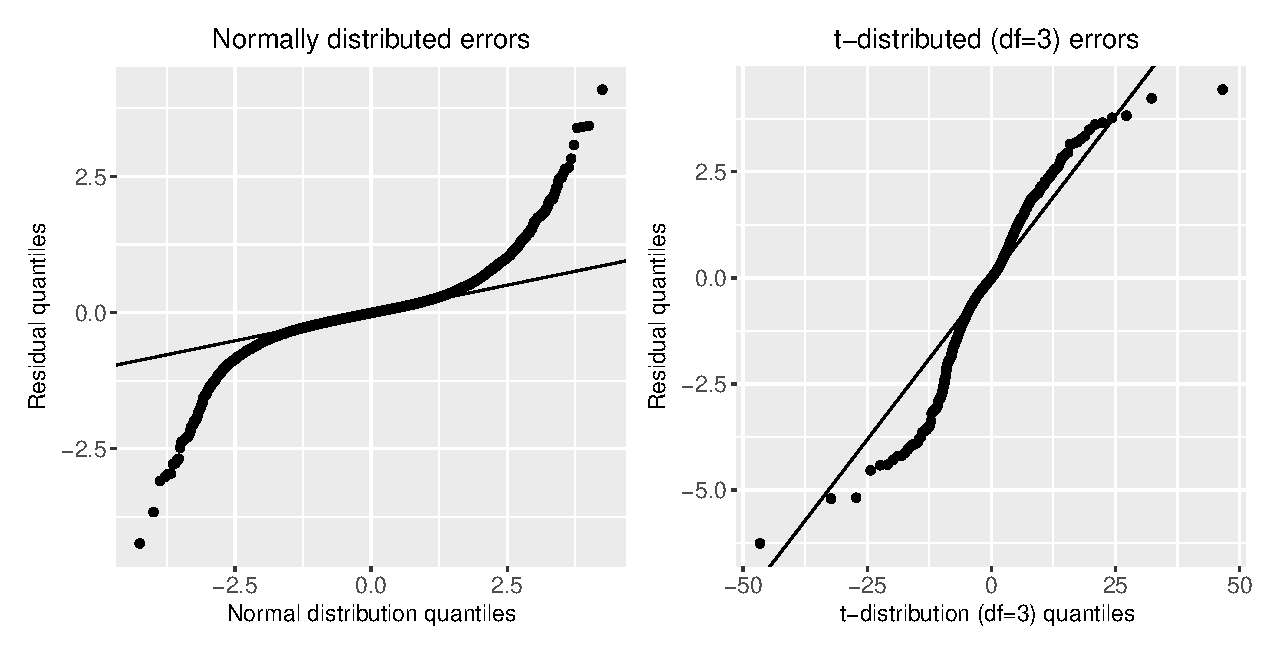
\includegraphics[width=\columnwidth]{images/model_fit/qqplot_norm_t3.eps}}
\caption{Quantile-quantile plots of subject specific residuals obtained from joint models with assumption of normally distributed errors, and t-distributed (df=3) errors, fitted to the PRIAS data set.}
\label{fig : qqplot_norm_t3_web}
\end{figure}

\clearpage

\subsection{Parameter Estimates}
\label{subsec : param_estimates}
The posterior parameter estimates for the joint model we fitted to the PRIAS dataset are shown in \ref{tab : PSA_long} (longitudinal sub-model) and \ref{tab : PSA_survival} (relative risk sub-model), and parameter estimates for the variance-covariance matrix from the longitudinal sub-model are the following:
\begin{equation*}
\bmath{D} = \begin{bmatrix}
       0.469 & 0.092 & -0.099 \\[0.3em]
       0.092 & 1.092 & 0.378 \\[0.3em]
       -0.099 & 0.378 & 0.898
     \end{bmatrix}
\end{equation*} 
For longitudinal sub-model parameter estimates, in \ref{tab : PSA_long} we can see that the age of the patient trivially affects the baseline $\log_2 \mbox{PSA}$ score. Since the longitudinal evolution of $\log_2 \mbox{PSA}$ is modeled with non-linear terms, the interpretation of the coefficients corresponding to time is not straightforward. In lieu of the interpretation, in Web Figure \ref{fig : fitted_trend_psa} we present the fitted marginal evolution of $\log_2 \mbox{PSA}$ over a period of 10 years for a hypothetical patient who was included in AS at the age of 70 years. In addition we present plots of observed versus fitted profiles for nine randomly selected patients (each with more than 3 observations) in Web Figure \ref{fig : subject_fittedVsObserved_psa_t3}.

\begin{figure}[!htb]
\centerline{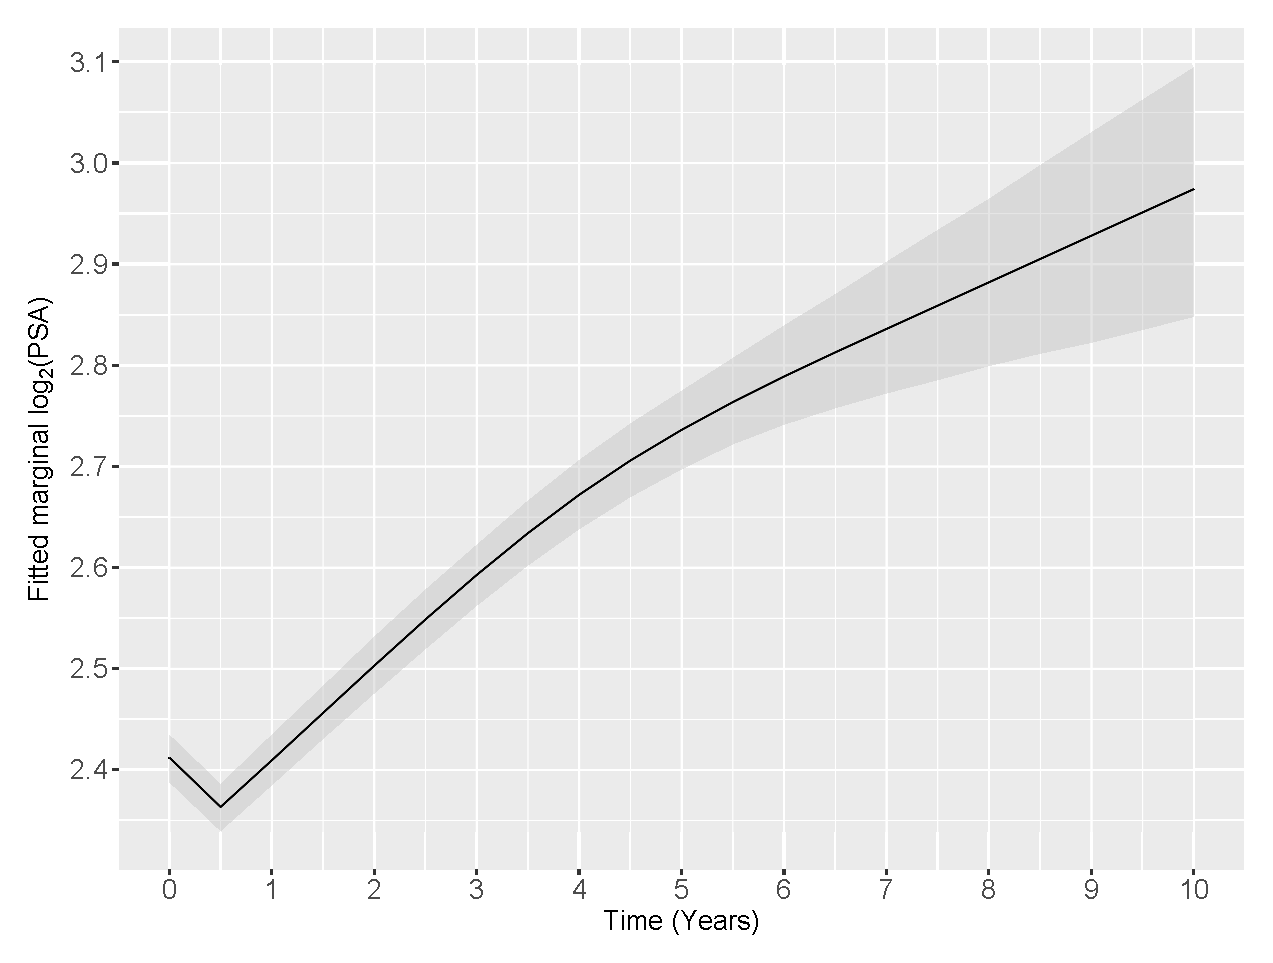
\includegraphics[width=\columnwidth]{images/model_fit/marginal_fitted_psa_t3.eps}}
\caption{Fitted marginal evolution of $\log_2 \mbox{PSA}$ over a period of 10 years with 95\% credible interval, for a hypothetical patient who was included in AS at the age of 70 years.}
\label{fig : fitted_trend_psa}
\end{figure}

\begin{figure}[!htb]
	\centerline{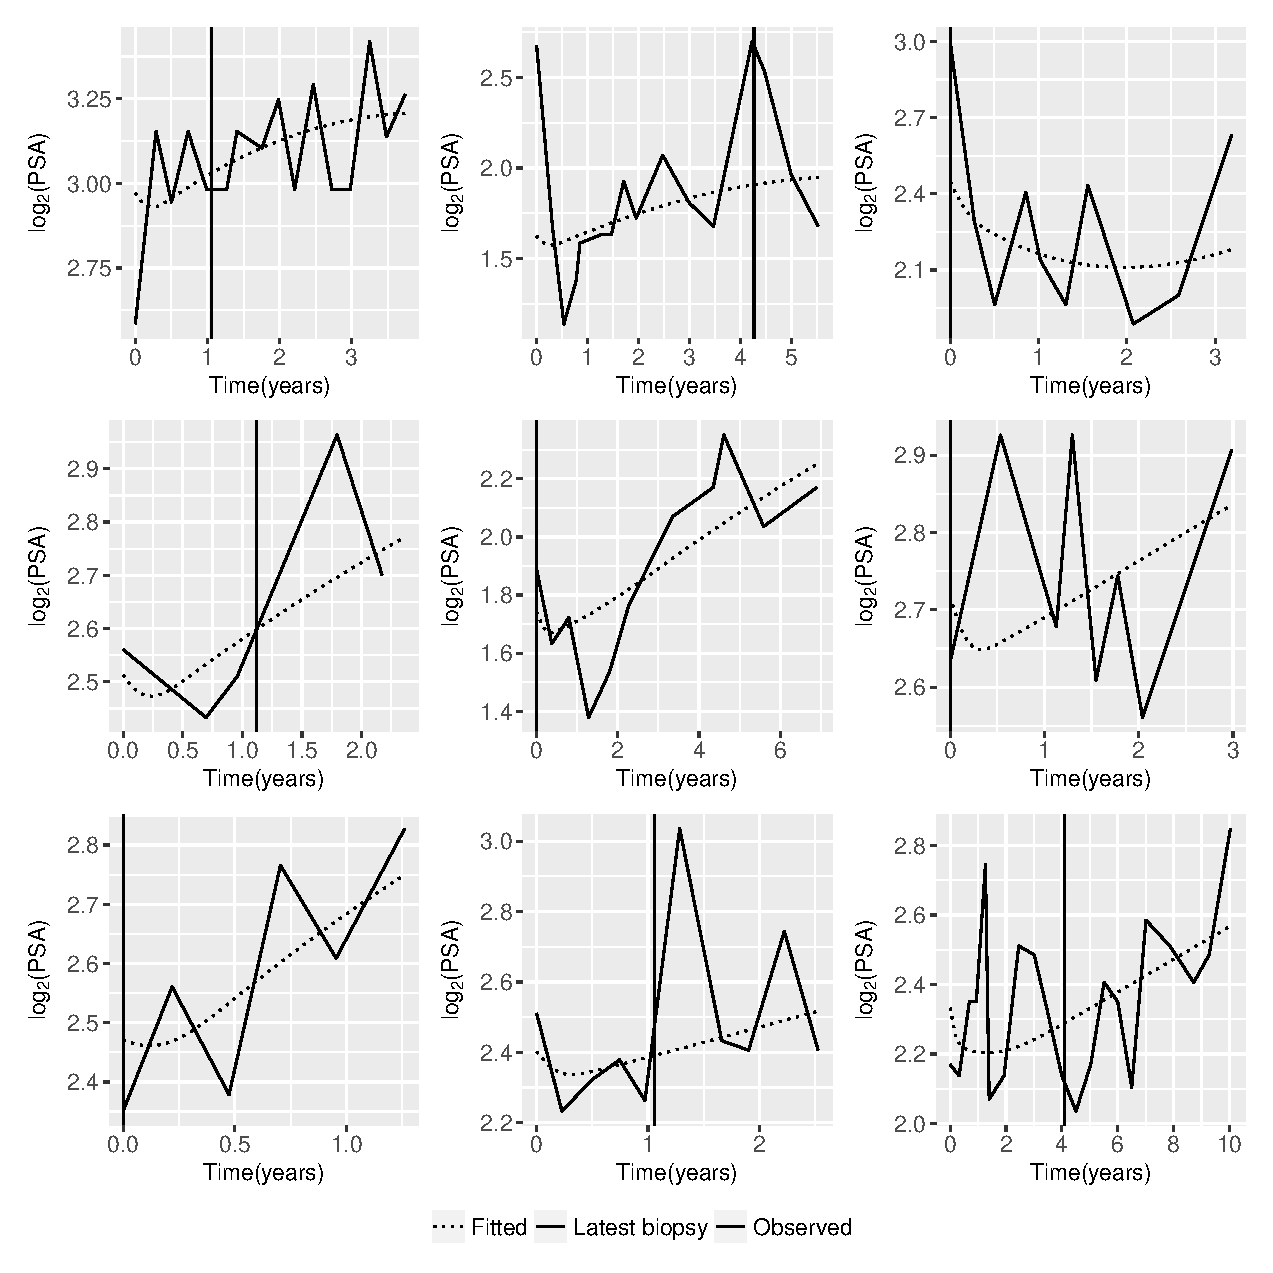
\includegraphics[width=\columnwidth]{images/model_fit/subject_fittedVsObserved_psa_t3.eps}}
	\caption{Fitted versus observed $\log_2 \mbox{PSA}$ profiles for nine randomly selected PRIAS patients. The fitted profiles utilize information from both the observed PSA levels and time of latest biopsy.}
	\label{fig : subject_fittedVsObserved_psa_t3}
	\end{figure}

\begin{table}[!htb]
\begin{center}
\caption{Estimated mean and 95\% credible interval for the parameters from the longitudinal sub-model of the joint model fitted to the PRIAS dataset.}
\label{tab : PSA_long}
\begin{tabular}{lrrrrr}
\Hline
Variable & Mean   & Std. Dev           & 2.5\%               & 97.5\%              & P              \\ \hline
Intercept                            &  2.412 & 0.012 & 2.388 & 2.435               & \textless0.000 \\
$(\mbox{Age} - 70)$                         & 0.003 & 0.001 & -3.039 $\times 10^{-4}$ & 0.005 & 0.084          \\
$(\mbox{Age} - 70)^2$       & -0.001 & 0.001 & -0.001 & -3.696 $\times 10^{-4}$ & \textless0.000 \\
Spline: visit time {[}0.0, 0.1{]} years   & 0.044 & 0.010 & 0.026 & 0.063 & \textless0.000 \\
Spline: visit time {[}0.1, 0.5{]} years & 0.297 & 0.015  &0.269 & 0.328           & \textless0.000 \\
Spline: visit time {[}0.5, 4.0{]} years & 0.316 & 0.025 &  0.270 & 0.364        & \textless0.000 \\
Spline: visit time {[}4.0, 7.0{]} years   & 0.466 & 0.032 & 0.402 & 0.527               & \textless0.000 \\
$\sigma$                               & 0.181 & 0.001 & 0.179 & 0.183              &  \\ \hline
\end{tabular}
\end{center}
\end{table}

\clearpage

For the relative risk sub-model, the parameter estimates in \ref{tab : PSA_survival} show that $\log_2 \mbox{PSA}$ velocity and the age at the time of inclusion in AS are strongly associated with the hazard of GR. For any patient, an increase in $\log_2 \mbox{PSA}$ velocity from -0.104 to 0.140 (first and third quartiles of the fitted velocities, respectively) corresponds to a 2.022 fold increase in the hazard of GR. An increase in age at the time of inclusion in AS from 65 years to 75 years (first and third quartiles of age in PRIAS dataset) corresponds to a 1.419 fold increase in the hazard of GR.

\begin{table}[!htb]
\begin{center}
\caption{Estimated mean and 95\% credible interval for the parameters of the relative risk sub-model of the joint model fitted to the PRIAS dataset.}
\label{tab : PSA_survival}
\begin{tabular}{lrrrrr}
\Hline
Variable                      & Mean   & Std. Dev & 2.5\%  & 97.5\%                 & P              \\ \hline
$(\mbox{Age} - 70)$                    & 0.035 & 0.006 & 0.023 & 0.047                  & \textless0.000 \\
$(\mbox{Age} - 70)^2$   & -0.001 & 0.001 & -0.003 & 1.364 $\times 10^{-4}$ & 0.084          \\
$\log_2 \mbox{PSA}$                  & -0.004 & 0.060 & -0.119 & 0.117 & 0.934         \\
Slope($\log_2 \mbox{PSA}$)           & 2.888 & 0.290 & 2.318 & 3.452 & \textless0.000 \\
\hline
\end{tabular}
\end{center}
\end{table}

\clearpage

To compare the predictive performance of a model having association between hazard of GR and $\log_2 \mbox{PSA}$ values, versus a model having the association with both $\log_2 \mbox{PSA}$ value and velocity, we calculate the area under the receiver operating characteristic curves, also called AUC \citep*{landmarking2017}, for these models. Since in a joint model time dependent AUC is more relevant, we calculate the AUC at year one, year two and year three of follow-up in AS. The time window for which the AUC is calculated is one year. The resulting AUC are presented in \ref{tab : AUC}.

\begin{table}[!htb]
\begin{center}
\caption{Area under the receiver operating characteristic curves (AUC), and 95\% confidence interval in brackets. AUC's are calculated for two joint models: first one having association between hazard of GR and $\log_2 \mbox{PSA}$ value as well as velocity, and second one having association with only $\log_2 \mbox{PSA}$ value.}
\label{tab : AUC}
\begin{tabular}{rrr}
\Hline
Year                      & $\log_2 \mbox{PSA}$ value and velocity association & $\log_2 \mbox{PSA}$ value association\\ 
\hline
1 & 0.613 [0.582, 0.632] & 0.595 [0.565, 0.618]\\
2 & 0.648 [0.608, 0.685] & 0.609 [0.568, 0.654]\\
3 & 0.593 [0.560, 0.638] & 0.590 [0.536, 0.628]\\
\hline
\end{tabular}	
\end{center}
\end{table}

\clearpage
\subsection{PSA-DT Dependent Interval Censoring in Time of Gleason Reclassification}
In PRIAS, the interval $l_i < T_i^* \leq r_i$ in which GR is detected depends on the observed PSA values (via PSA-DT). It is natural to question in this scenario if the parameters of the joint model are affected by PSA-DT dependent interval censoring. To this end, we discussed via the formulation of the likelihood function in \ref{subsec : int_censoring_fulllikelihood_proof}, that the joint model gives consistent and asymptotically unbiased estimates of the parameters even if the interval censoring depends on PSA-DT, under the condition that the model is correctly specified. However, in this section we also demonstrate this via a simulated dataset of 750 patients. The true event times $T^*_i$ for these patients were generated using parameters from a joint model fitted to the PRIAS dataset. However this joint model did not include association between velocity of log PSA values and hazard of GR. That is, the hazard of GR $h_i(t)$ at any time $t$ depends only on the underlying log PSA value $m_i(t)$ at that time. Furthermore, for these patients we used the schedule of PRIAS to generate the interval $l_i \leq T^*_i \leq r_i$ in which GR is detected. Thus the observed data for $i$-th patient is $\{\boldsymbol{y}_i, l_i, r_i\}$. Our aim is to show that if there is no association between $h_i(t)$ and velocity of log PSA value $m'_i(t)$, then even though the biopsy schedule depends on PSA-DT (which is a crude measure of PSA velocity), a joint model fitted with both value and velocity associations will have an insignificant velocity association. In the fitted joint model we found the value association (95\% credible interval in brackets) to be 0.182 [0.090, 0.274], and the velocity association to be -0.001 [-0.295, 0.254]. That is even though the schedule of biopsies depended upon observed PSA values it did not lead to a spurious velocity association. To check if we correctly specified the joint model, we performed several sensitivity analysis in our model (e.g., changing the position of the knots, etc.) to investigate the fit of the model and also the robustness of the results. In all of our attempts, the same conclusions were reached, namely that the $\log_2 \mbox{PSA}$ velocity is more strongly associated with the hazard of GR compared to the $\log_2 \mbox{PSA}$ levels.
\clearpage
% !TEX root =  ../supplementary.tex

\section{Personalized Schedules for the Demonstration Patients from PRIAS.}
\label{sec : demo_3174_2340}

In this section we demonstrate the application of personalized schedules on patients from PRIAS study. In Section \ref{subsec : demo_prias_pers_schedule} of the main manuscript we demonstrated personalized schedules for the first demonstration patient. Here we demonstrate them for the remaining two patients.

The evolution of PSA, repeat biopsy history and proposed times of biopsies for the second demonstration patient are shown in the top panel of Web Figure \ref{fig : prias_demo_pid_3174}. It can be seen that the schedule of biopsy based on expected time of GR adjusts the times of biopsy according to the rise in hazard, which increases due to steep rise in $\log_2 \mbox{PSA}$ velocity. More specifically, at year two the proposed biopsy time is 12.5 years whereas at year four it decreases to 5.3 years. On average, a biopsy scheduled using expected time of GR at year two should have a larger offset $O^S_j$ compared to the same at year four. This is because the standard deviation of $g(T^*_j)$, given by $\mbox{SD}_g(T^*_j) = \sqrt{\mbox{var}_g(T^*_j)}$, is considerably lower at year four as shown in the bottom panel of Web Figure \ref{fig : prias_demo_pid_3174}. In the figure it can be seen that the standard deviation decreases with sharp increase in PSA. As for the schedules based on dynamic risk of GR, the threshold $\kappa$ was automatically chosen using $\mbox{F}_1$ score, and was estimated to be between 1 and 0.9 at all time points. This value of $\kappa$ corresponds to a time very close to the time of latest biopsy ($t=0$). Hence the biopsies are scheduled much earlier than those based on expected time of GR.

\begin{figure}
\centerline{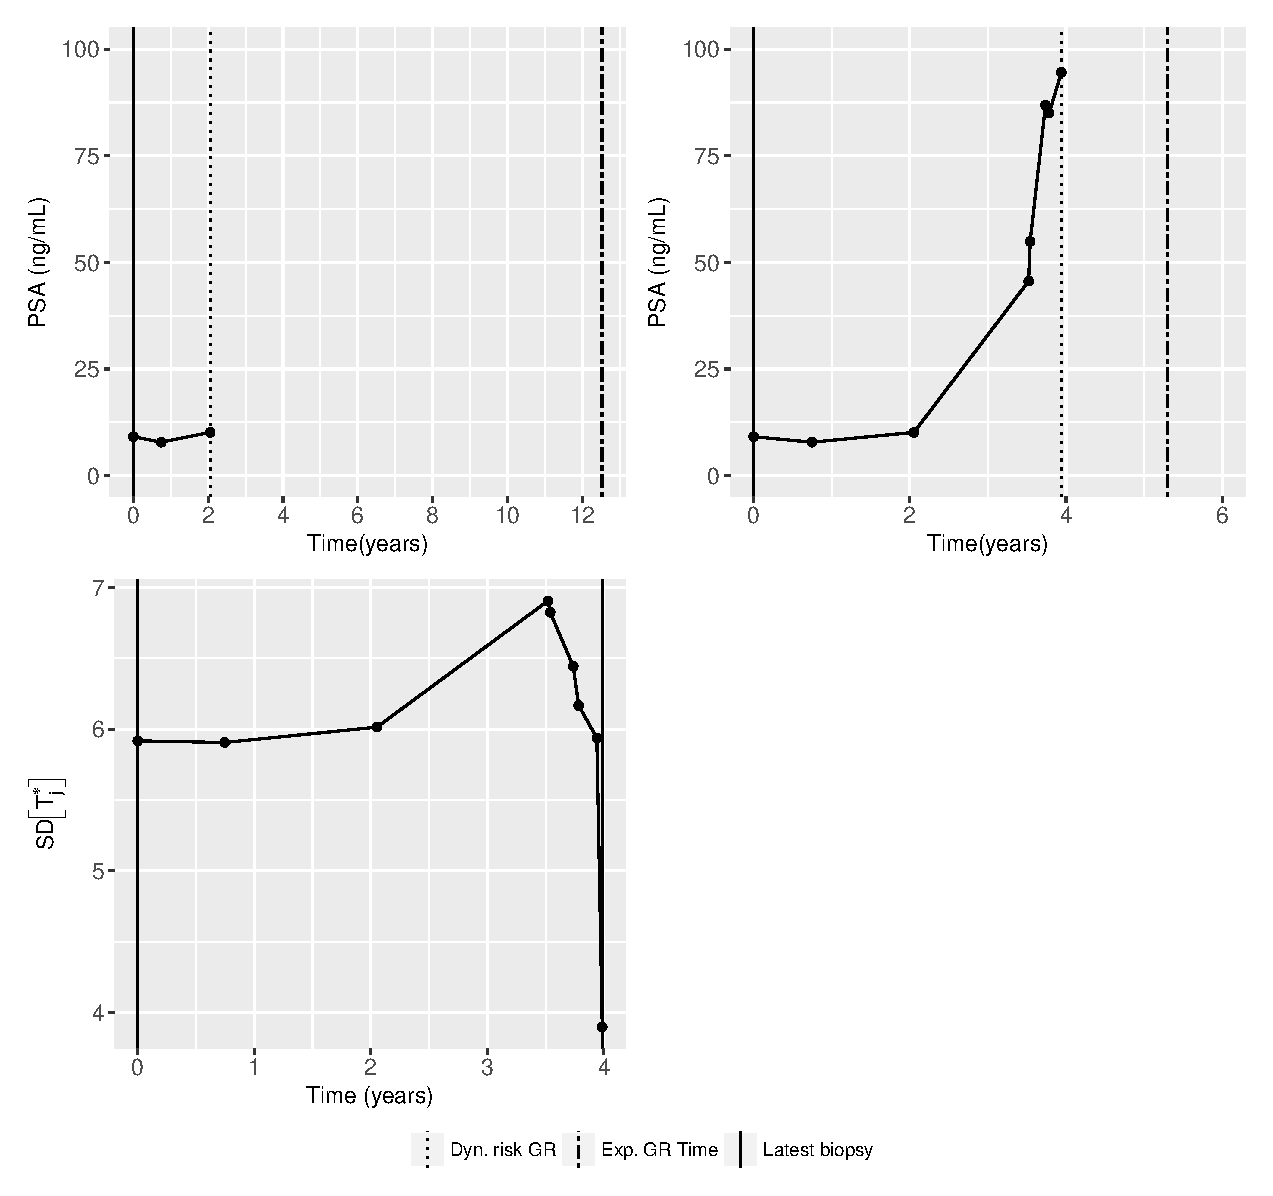
\includegraphics[width=\columnwidth]{images/prias_demo/case_3174.eps}}
\caption{Top panel: Evolution of PSA, history of repeat biopsies and corresponding personalized schedules for the second demonstration patient. Bottom Panel: History of repeat biopsies and $\mbox{SD}_g(T^*_j) = \sqrt{\mbox{var}_g(T^*_j)}$ over time for the second demonstration patient.}
\label{fig : prias_demo_pid_3174}
\end{figure}

\clearpage

Patient 2340 presents a case where information from PSA levels and repeat biopsies is conflicting. In Web Figure \ref{web_fig : prias_demo_pid_2340} we can see that the PSA for this patient increased by 100\% between year two and year 3.2. If only information from PSA is considered, then we can see that proposed time of biopsy based on expected time of GR is preponed from 14.6 to 13.0 years during this period. However, if we also take into account the negative result from the repeat biopsy at year 2.5, then the proposed time of biopsy is postponed from 14.6 years to 15 years. Thus more weight is given to a recent negative biopsy result than PSA, which is in accordance with the clinical practice. The proposed time of biopsy based on dynamic risk of GR is also postponed from 2.3 to 3.6 years in light of the negative biopsy result.

\begin{figure}
\centerline{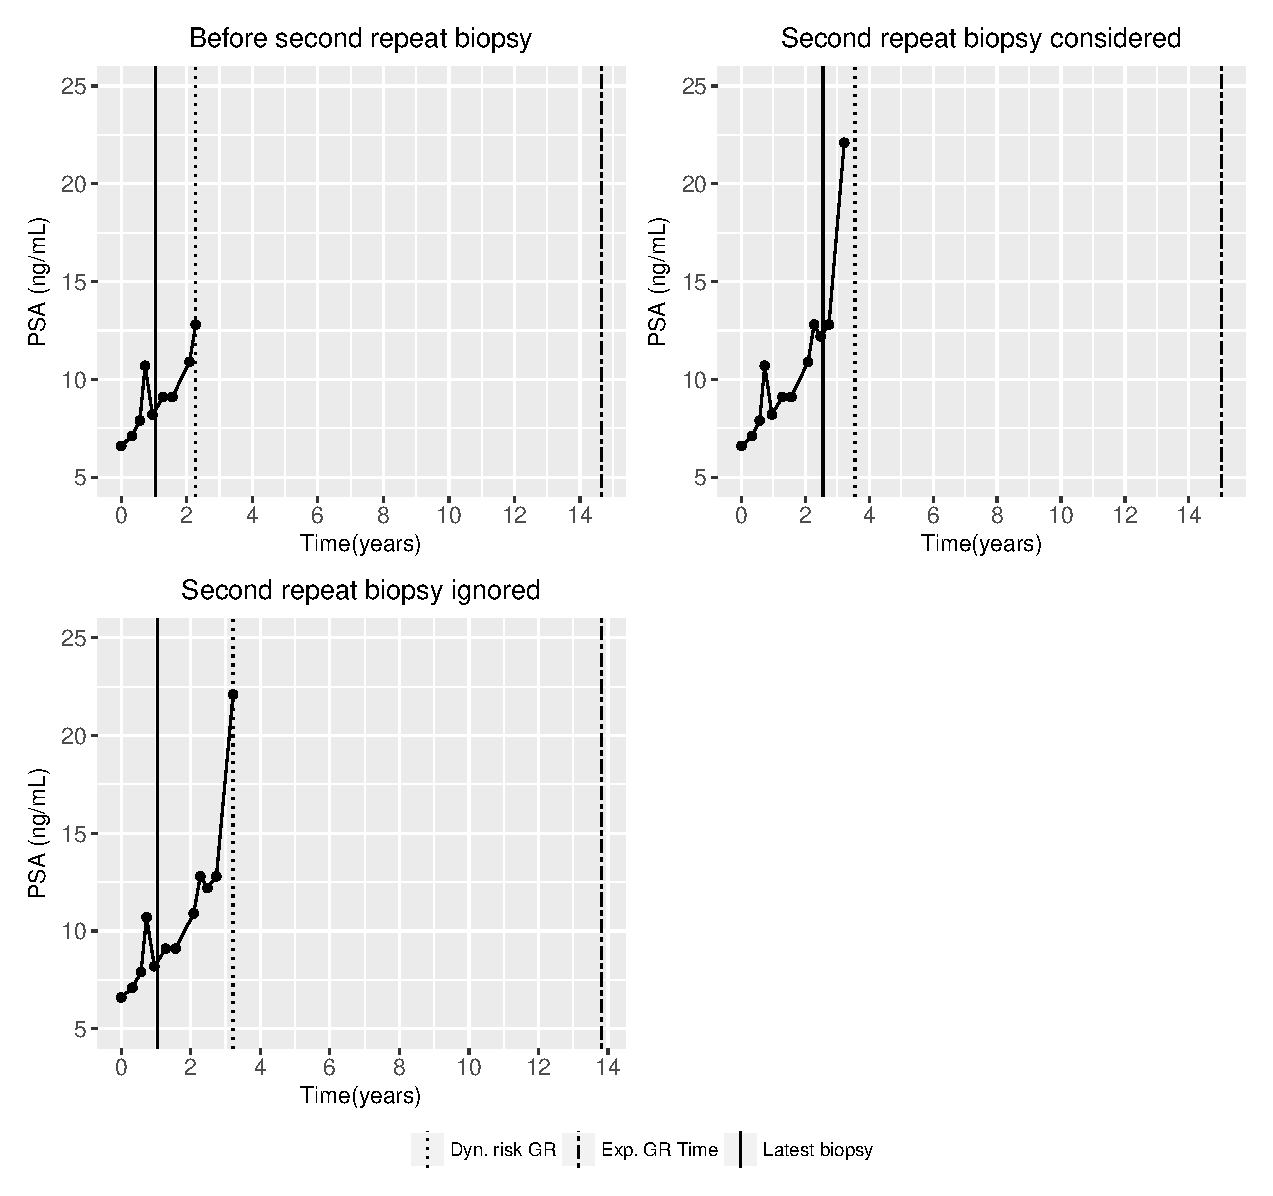
\includegraphics[width=\columnwidth]{images/prias_demo/case_2340.eps}}
\caption{Evolution of PSA, history of repeat biopsies and corresponding personalized schedules for the third demonstration patient.}
\label{web_fig : prias_demo_pid_2340}
\end{figure}
\clearpage
% !TEX root =  ../supplementary.tex
\section{Simulation Study}
\subsection{Simulation Results for Dynamic Risk of GR Based Approach With a Fixed $\kappa = 0.95$}
In the main manuscript, for the personalized schedules based on dynamic risk of GR we chose $\kappa$ on the basis of $\mbox{F}_1$ score. However while conducting the simulation study, we also tried a fixed $\kappa$ of 0.95, which means that the next biopsy is scheduled at a time point where the dynamic risk of GR is 5\%. The results for this approach are presented in \ref{table : sim_study_pooled_estimates_extended}. In the table, the abbreviation Dyn. risk GR ($\mbox{F}_1$ score) corresponds to personalized schedules based on dynamic risk of GR based approach, with $\kappa$ chosen on the basis of $\mbox{F}_1$ score. The abbreviation Hybrid ($\mbox{F}_1$ score) corresponds to the hybrid approach between median time of GR and dynamic risk of GR ($\kappa$ chosen on the basis of $\mbox{F}_1$ score).

\begin{table}[!htb]
\caption{Estimated mean and standard deviation (SD), of the number of biopsies $N^S_j$ conducted until Gleason reclassification (GR) is detected, and of the offset $O^S_j$ (difference in time at which GR is detected and the true time of GR, in months), for the simulated (500 datasets) test patients, across different schedules and subgroups. Patients in subgroup $G_1$ have the fastest prostate cancer progression rate, whereas patients in subgroup $G_3$ have the slowest progression rate. Types of personalized schedules (full names in brackets): Exp. GR Time (expected time of GR), Med. GR Time (median time of GR), Dyn. risk GR (schedules based on dynamic risk of GR), Hybrid (a hybrid approach between median time of GR and dynamic risk of GR). Annual corresponds to a schedule of yearly biopsies and PRIAS corresponds to biopsies as per PRIAS protocol.}
\label{table : sim_study_pooled_estimates_extended}
\begin{tabular}{lrrrr}
\Hline
\multicolumn{5}{c}{a) All hypothetical subgroups}\\
\hline
Schedule          & $E(N^S_j)$ & $E(O^S_j)$ & ${\mbox{SD}(N^S_j)}$ & ${\mbox{SD}(O^S_j)}$ \\
\hline
Annual         & 5.24            & 6.01                & 2.53          & 3.46              \\
PRIAS          & 4.90            & 7.71                & 2.36          & 6.31\\
Dyn. risk GR ($\mbox{F}_1$ score)       & 4.69            & 6.66                & 2.19           & 4.38              \\
Hybrid ($\mbox{F}_1$ score)      & 3.75            & 9.70                & 1.71          & 7.25              \\
Dyn. risk GR ($\kappa=0.95$) & 5.15 & 6.02 & 2.51 & 3.47\\
Med. GR time & 2.06            & 13.88               & 1.41          & 11.80              \\
Exp. GR time & 1.92            & 15.08               & 1.19          & 12.11             \\
\hline
\multicolumn{5}{c}{b) Hypothetical subgroup $G_1$}\\
\hline
Schedule        & $E(N^S_j)$ & $E(O^S_j)$ & ${\mbox{SD}(N^S_j)}$ & ${\mbox{SD}(O^S_j)}$ \\
\hline
Annual         & 4.32            & 6.02                & 3.13          & 3.44              \\
PRIAS          & 4.07            & 7.44                & 2.88          & 6.11    \\
Dyn. risk GR ($\mbox{F}_1$ score)       & 3.85            & 6.75                & 2.69          & 4.44              \\
Hybrid ($\mbox{F}_1$ score)       & 3.25            & 10.25               & 2.16          & 8.07              \\
Dyn. risk GR ($\kappa=0.95$) & 4.23 & 6.05 & 3.10 & 3.46\\
Med. GR time & 1.84            & 20.66               & 1.76          & 14.62             \\
Exp. GR time & 1.72            & 21.65               & 1.47          & 14.75             \\
\hline      
\multicolumn{5}{c}{c) Hypothetical subgroup $G_2$}\\
\hline
Schedule        & $E(N^S_j)$ & $E(O^S_j)$ & ${\mbox{SD}(N^S_j)}$ & ${\mbox{SD}(O^S_j)}$ \\
\hline
Annual         & 5.18            & 5.98                & 2.13          & 3.47              \\
PRIAS          & 4.85            & 7.70                & 2.00          & 6.29        \\
Dyn. risk GR ($\mbox{F}_1$ score)       & 4.63            & 6.66                & 1.82          & 4.37              \\
Hybrid ($\mbox{F}_1$ score)       & 3.68            & 10.32                & 1.37          & 7.45              \\
Dyn. risk GR ($\kappa=0.95$) & 5.09 & 5.99 & 2.11 & 3.47\\
Med. GR time & 1.89             & 12.33               & 1.16          & 9.44              \\
Exp. GR time & 1.77            & 13.54               & 0.98          & 9.83              \\
\hline      
\multicolumn{5}{c}{d) Hypothetical subgroup $G_3$}\\
\hline
Schedule        & $E(N^S_j)$ & $E(O^S_j)$ & ${\mbox{SD}(N^S_j)}$ & ${\mbox{SD}(O^S_j)}$ \\
\hline
Annual         & 6.20             & 6.02                & 1.76          & 3.46              \\
PRIAS          & 5.76             & 7.98                & 1.71         & 6.51        \\
Dyn. risk GR ($\mbox{F}_1$ score)       & 5.58            & 6.58                & 1.56          & 4.33              \\
Hybrid ($\mbox{F}_1$ score)       & 4.32            & 8.55                & 1.26          & 5.91              \\
Dyn. risk GR ($\kappa=0.95$) & 6.11 & 6.01 & 1.76 & 3.46\\
Med. GR time & 2.45            & 8.70                & 1.15          & 6.32              \\
Exp. GR time & 2.27            & 10.09               & 0.99          & 7.47              \\
\hline     
\end{tabular}
\end{table}

\clearpage

\subsection{Variation in Estimated Mean and Standard Deviation, of Number of Biopsies and Offset Across the 500 Simulations}
In this section we present figures related to the simulation study results discussed in Section \ref{sec: simulation_study} of main manuscript. The figures we present next are population specific, i.e. subgroup level differentiation is not done.

\begin{itemize}
  \item Variation in estimated mean across the 500 simulations, for number of biopsies and offset (difference in time at which Gleason reclassification or GR is detected and the true time of GR, in months) for different methods is shown in Web Figure \ref{fig : nbMeanBoxPlot_all} and Web Figure \ref{fig : offsetMeanBoxPlot_all}.
  \item Variation in estimated standard deviation across the 500 simulations, for number of biopsies and offset (difference in time at which Gleason reclassification or GR is detected and the true time of GR, in months) for different methods is shown in Web Figure \ref{fig : nbSDBoxPlot_all} and Web Figure \ref{fig : offsetSDBoxPlot_all}.
\end{itemize}

\begin{figure}[!htb]
\centerline{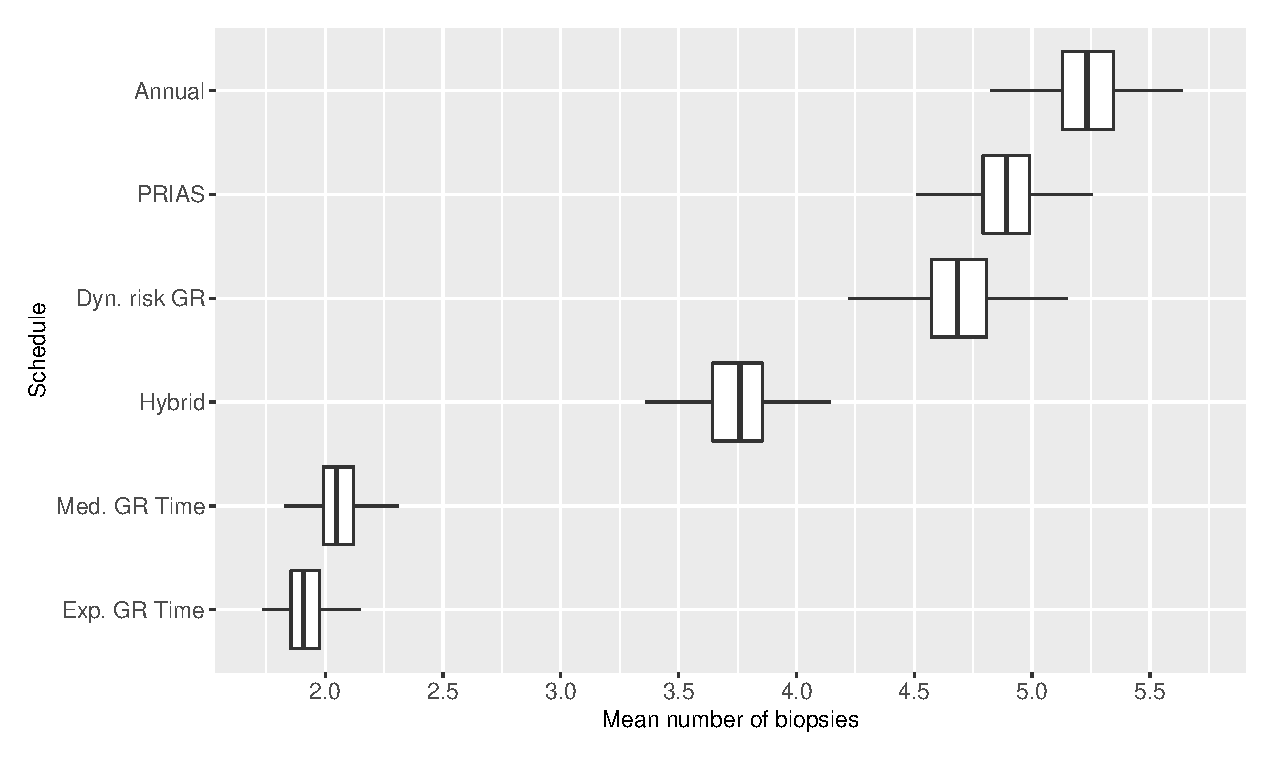
\includegraphics[width=\columnwidth]{images/sim_study/nbMeanBoxPlot_all.eps}}
\caption{Boxplot showing variation in estimated mean number of biopsies conducted by various schedules until Gleason reclassification is detected, obtained from the simulation study with 500 simulated datasets.}
\label{fig : nbMeanBoxPlot_all}
\end{figure}

\begin{figure}[!htb]
\centerline{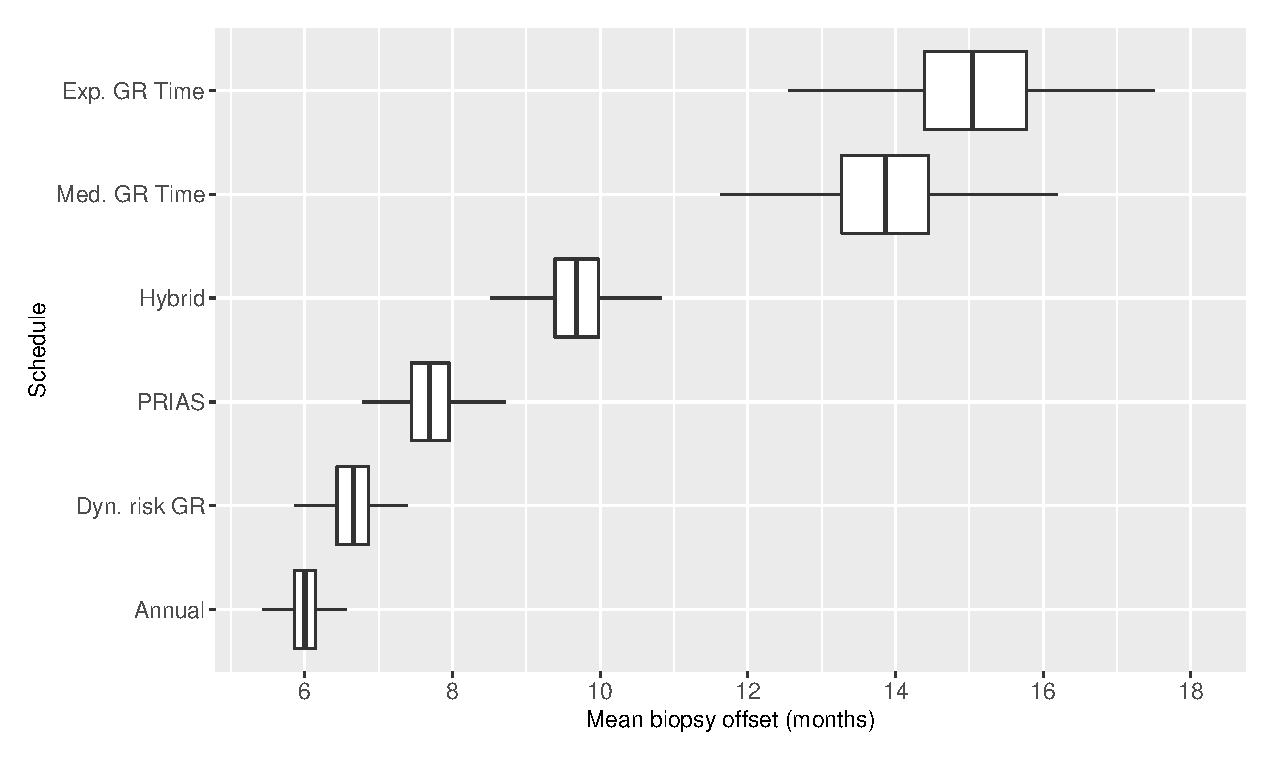
\includegraphics[width=\columnwidth]{images/sim_study/offsetMeanBoxPlot_all.eps}}
\caption{Boxplot showing variation in estimated mean of biopsy offset (difference in time at which Gleason reclassification or GR is detected and the true time of GR, in months) for various schedules, obtained from the simulation study with 500 simulated datasets.}
\label{fig : offsetMeanBoxPlot_all}
\end{figure}

\begin{figure}[!htb]
\centerline{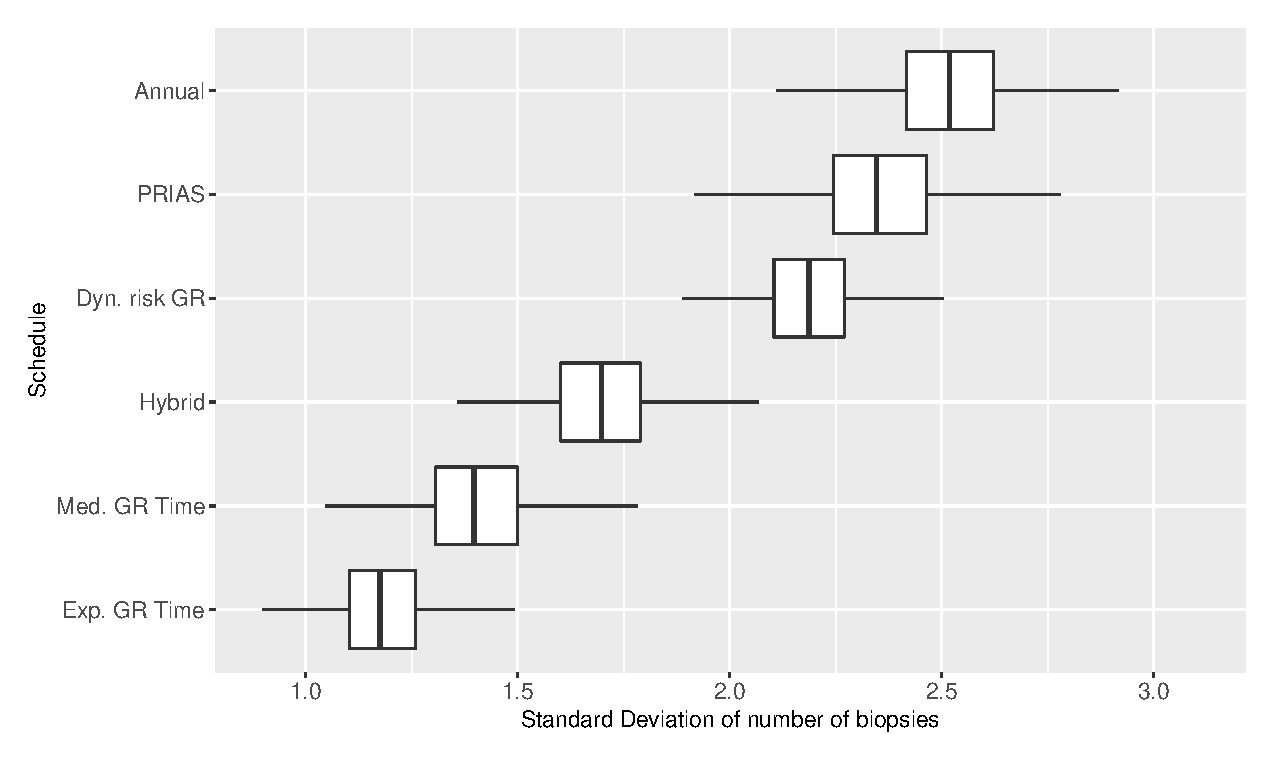
\includegraphics[width=\columnwidth]{images/sim_study/nbSDBoxPlot_all.eps}}
\caption{Boxplot showing variation in estimated standard deviation of number of biopsies conducted by various schedules until Gleason reclassification is detected, obtained from the simulation study with 500 simulated datasets.}
\label{fig : nbSDBoxPlot_all}
\end{figure}

\begin{figure}[!htb]
\centerline{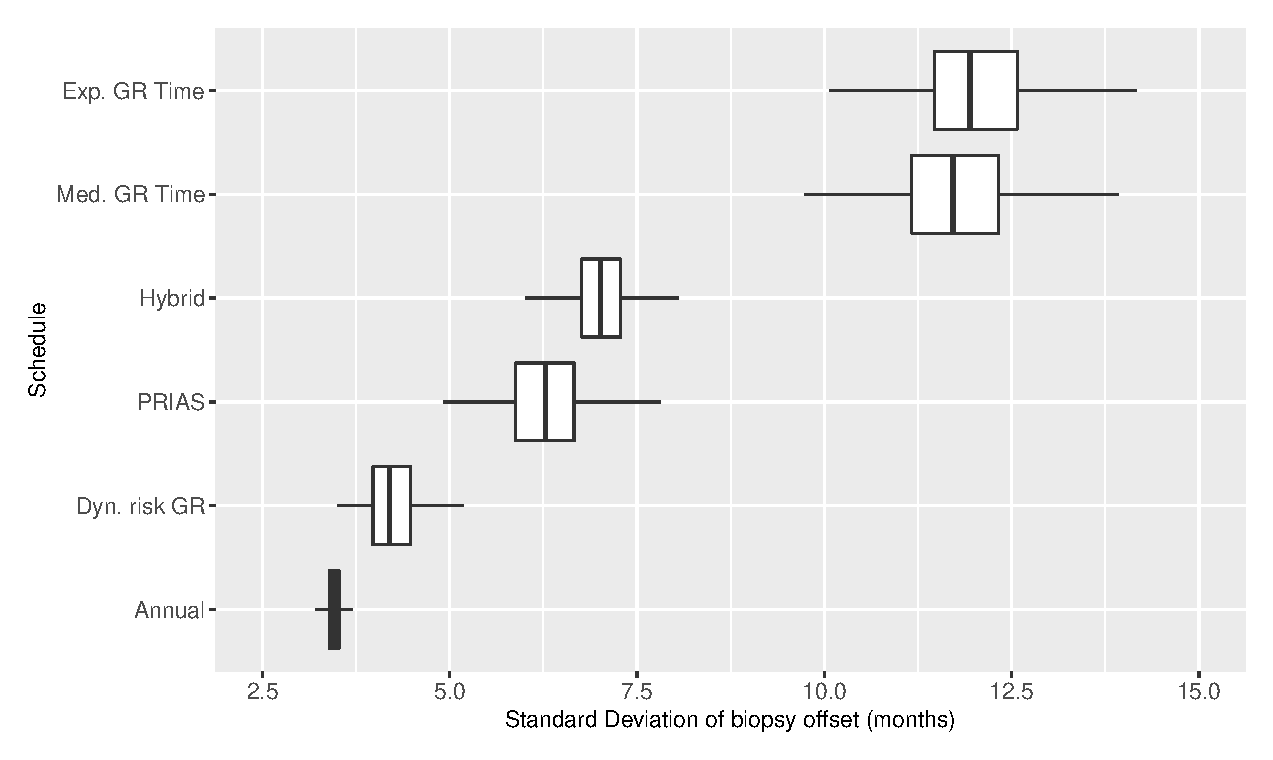
\includegraphics[width=\columnwidth]{images/sim_study/offsetSDBoxPlot_all.eps}}
\caption{Boxplot showing variation in estimated standard deviation of biopsy offset (difference in time at which Gleason reclassification or GR is detected and the true time of GR, in months) for various schedules, obtained from the simulation study with 500 simulated datasets.}
\label{fig : offsetSDBoxPlot_all}
\end{figure}




\clearpage
% !TEX root =  ../supplementary.tex
\section{Source Code}
The R code for fitting the joint model to the PRIAS dataset, and for the simulation study are available at \url{https://github.com/anirudhtomer/prias/tree/master/src/decision_analytic}. We refer to this location as `DATA\_HOME' in the rest of this document.

\subsection{Fitting the joint model to the PRIAS dataset}
\textbf{Accessing the dataset:}
The PRIAS dataset is not openly accessible. However, access to the database can be requested via the contact links at \url{www.prias-project.org}.\\

\textbf{Formatting the dataset:}
This dataset however is in the so-called wide format and also requires removal of incorrect entries. This can be done via the R script \url{DATA_HOME/fittingModel/dataset_cleaning.R}. This will lead to two R objects, namely `prias.id' and `prias\_long'. The `prias.id' object contains information about time of cancer progression for PRIAS patients. The `prias\_long' object contains longitudinal PSA, DRE measurements, time of biopsies and results of biopsies.\\

\textbf{Fitting the joint model:}
We use a joint model for time to event and bivariate longitudinal data to model the evolution of PSA and DRE measurements over time, and to simultaneously model their association with the risk of cancer progression. The R package we use for this purpose is called \textbf{JMbayes} (https://cran.r-project.org/web/packages/JMbayes/JMbayes.pdf). The API we use, however, are currently not hosted on CRAN, and can be found here:
\url{https://github.com/drizopoulos/JMbayes}. The joint model can be fitted via the script \url{DATA_HOME/fittingModel/psa_dre_jointAnalysis.R}. It takes roughly 6 hours to run on an Intel core-i5 machine with 4 cores, and 8GB of RAM. 

The graphs presented in the main manuscript, and the supplementary material can be generated by the scripts \url{DATA_HOME/fittingModel/demographs.R}, and \url{DATA_HOME/fittingModel/modelDiagnostic.R}, respectively.

\subsection{Running the simulation study}
The simulation study can be run by the following script: \url{DATA_HOME/simulationStudy/controller.R}. Although it depends on other files, the code should run without errors as long as the directory structure is maintained. An entire simulation study may take weeks to run. However, this can be controlled via the variable `dataSetNums' in the script. Graphs related to simulation study results can be generated from the scripts \url{DATA_HOME/simulationStudy/decisionMakingGraph.R} and \url{DATA_HOME/simulationStudy/produceResults.R} 
\clearpage
%  The \backmatter command formats the subsequent headings so that they
%  are in the journal style.  Please keep this command in your document
%  in this position, right after the final section of the main part of 
%  the paper and right before the Acknowledgements, Supplementary Materials,
%  and References sections. 

\backmatter

%  Here, we create the bibliographic entries manually, following the
%  journal style.  If you use this method or use natbib, PLEASE PAY
%  CAREFUL ATTENTION TO THE BIBLIOGRAPHIC STYLE IN A RECENT ISSUE OF
%  THE JOURNAL AND FOLLOW IT!  Failure to follow stylistic conventions
%  just lengthens the time spend copyediting your paper and hence its
%  position in the publication queue should it be accepted.

%  We greatly prefer that you incorporate the references for your
%  article into the body of the article as we have done here 
%  (you can use natbib or not as you choose) than use BiBTeX,
%  so that your article is self-contained in one file.
%  If you do use BiBTeX, please use the .bst file that comes with 
%  the distribution.  In this case, replace the thebibliography
%  environment below by 
%
%  \bibliographystyle{biom} 
% \bibliography{mybibilo.bib}
\bibliographystyle{biom} 
\bibliography{bibliography}

\label{lastpage}

\end{document}
